% !TEX encoding = UTF-8
% !TEX TS-program = pdflatex
% !TEX root = ../Volpe_Andrea.tex

%**************************************************************
\chapter{Progettazione}
\label{cap:progettazione}

\intro{In questo capitolo viene descritta la fase di progettazione effettuata per
la realizzazione del progetto.}

% %**************************************************************
\section{Architettura del progetto}
Questo progetto è nato con lo scopo di fare un'analisi
comparativa con un progetto già esistente. Per rendere 
l'analisi comparativa più efficace, è stato scelto di usare la stessa architettura dell'altro progetto, 
ovvero la layered architecture.
\\\\
Questo tipo di architettura velocizza la realizzazione del progetto, a discapito della facilità di
manutenzione ma non è un problema dato che le dimensioni del prodotto al momento sono contenute. Se
le dimensioni del progetto dovessero aumentare notevolmente, fino al punto in cui il processo di manutenzione risulti 
difficile, è possibile
migrarlo a un'architettura a microservizi in qualsiasi momento.

% ref: https://cs.uwaterloo.ca/~m2nagapp/courses/CS446/1195/Arch_Design_Activity/Layered.pdf

\subsection{Layered architecture}
La layered architecture è uno degli stili architetturali più utilizzati al giorno d'oggi. L'idea che sta dietro a
questo tipo di architettura consiste nell'organizzare i moduli o le componenti con funzionalità simili
in livelli orizzontali. Di conseguenza ogni livello svolge un ruolo specifico nell'applicazione.
\\
La layered architecture non ha restrizioni sul numero di strati che l'applicazione può avere, in quanto 
lo scopo è avere livelli che promuovano il concetto di separazione delle responsabilità.
\clearpage
\begin{figure}[H]
    \centering
    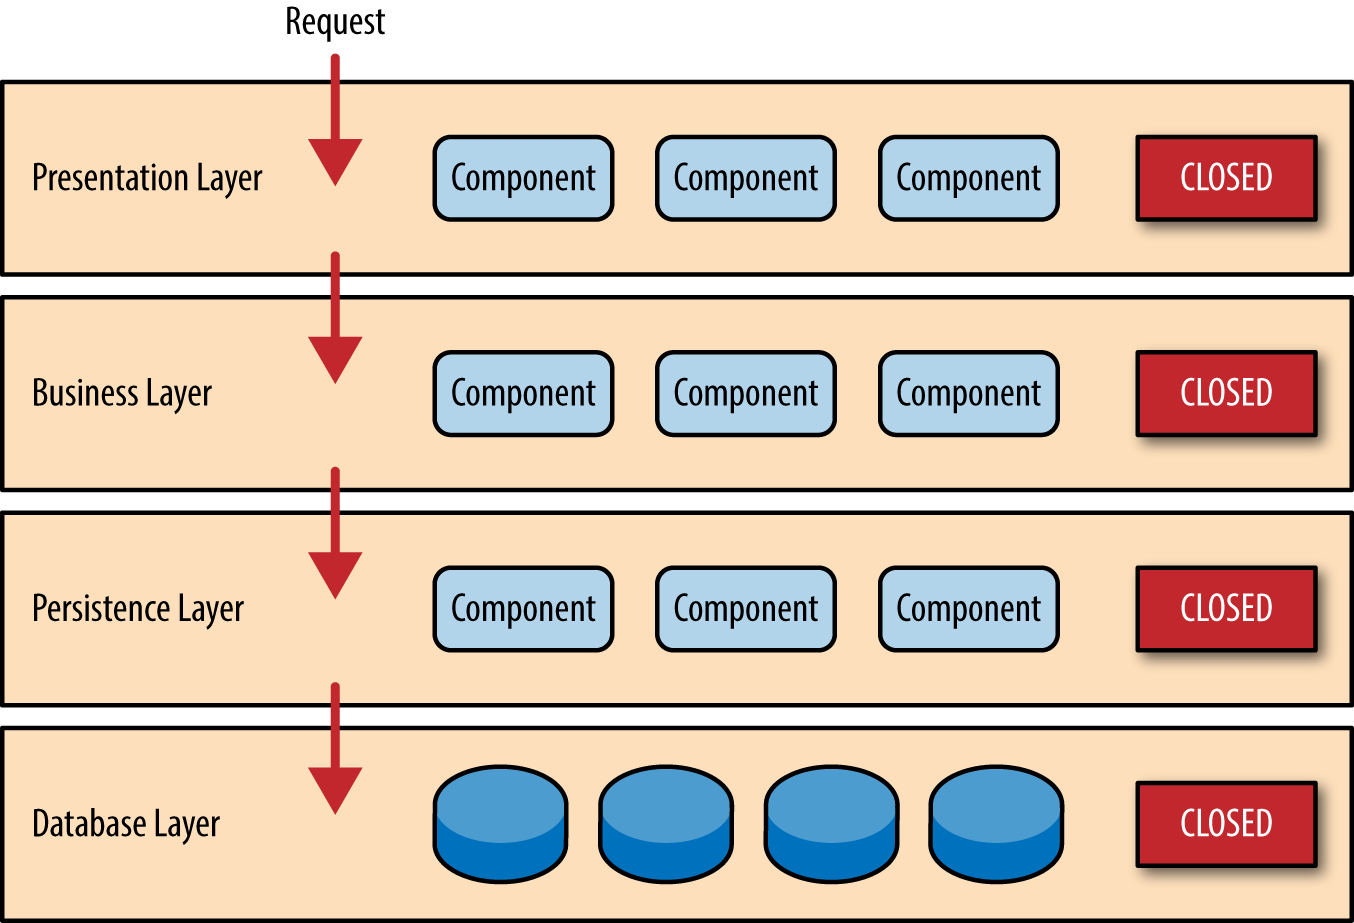
\includegraphics[height=5cm]{layered-architecture}
    \caption{Layered architecture}
\end{figure}
\leavevmode\newline
Solitamente ogni livello comunica solo con il livello sottostante. Il connettore tra ogni livello può 
essere una chiamata di funzione, una richiesta di query, un oggetto dati o qualsiasi connettore che
trasmetta richieste o informazioni.
\\
La denominazione dei livelli è abbastanza flessibile ma di solito sono sempre presenti almeno: un livello di presentazione, un livello
di business e un livello fisico.
\\\\\\
\textbf{Livello di presentazione}
\\\\
Il livello di presentazione contiene tutte le classi responsabili di presentare la visualizzazione delle
delle informazioni all'utente finale. Idealmente questo è il solo livello con cui l'utente finale 
interagisce direttamente.
\\\\\\
\textbf{Livello di business}
\\\\
Il livello di business contiene tutta la logica che è richiesta dall'applicazione per poter soddisfare i 
suoi requisiti funzionali. Solitamente questo livello si occupa dell'aggregazione, della computazione
e della richiesta dei dati. Quindi qui è dove viene implementata la logica principale dell'applicazione.
\\\\\\
\textbf{Livello fisico}
\\\\
Nel livello fisico sono salvati tutti i dati recuperabili dell'applicazione. Solitamente questo livello è chiamato
anche livello di persistenza. Si occupa di interagire con il sistema in cui i dati 
sono persistiti, ad esempio un database.
\subsection{Motivazioni della scelta}
Le motivazioni e i vantaggi che hanno portato a scegliere questo stile architetturale sono i seguenti:
\begin{itemize}
    \item dato che la separazione delle responsabilità è la proprietà principale di questa architettura,
        ogni livello software ha la sua specifica funzione. Questo rende facile aggiornare 
        separatamente i livelli e permette al team di sviluppo di suddividere i carichi di lavoro tra i 
        membri del team, che possono lavorare in contemporanea su componenti diverse;
    \item per la proponente era importante avere una suite di test automatici per testare le varie componenti
        dell'applicazione. La layered architecture
        permette di suddividere l'applicazione in componenti ben separate e quindi facili da testare.
        Essendo ogni livello isolato, è possibile creare casi di test di dimensione ridotte, 
        in quanto le componenti di cui fare il \gls{mock} sono poche;
    \item nel caso le dimensioni dell'applicazioni diventino importanti, è possibile, senza troppo sforzo, avviare un processo
        di migrazione ad un'architettura a microservizi. La layered architecture lavora bene (lato monolite) anche
        in un sistema con un'architettura ibrida monolite/microservizi. Questo tipo di architettura
        ibrida solitamente si viene a formare nel processo di migrazione di un sistema monolitico a un sistema a microservizi.
        \\
        Di conseguenza, in un ottica di futura migrazione a un sistema a microservizi (molto probabile che avvenga), è
        bene scegliere un monolite che lavori bene in un'architettura ibrida e quindi che sia facile da migrare.
        \\
        Infatti grazie alla separazione delle responsabilità e l'isolamento della layered architecture, è facile andare
        a trasformare le componenti del monolite in microservizi.
\end{itemize}
\clearpage
\section{Struttura software}
E' stato scelto NestJS come framework di sviluppo del progetto dato che utilizza la layered architecture
tramite il design pattern controller-service-repository. Vediamo questo design pattern:
\begin{figure}[H]
    \centering
    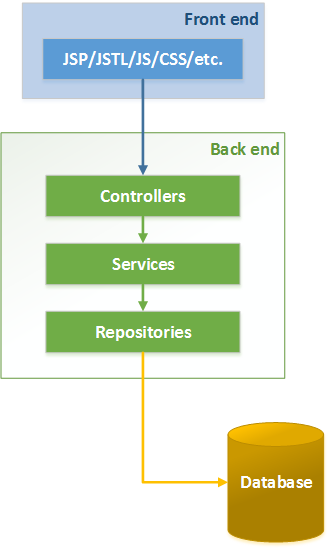
\includegraphics[height=9cm]{controller-service-repository-pattern}
    \caption{Controller-service-repository pattern}
\end{figure}
\leavevmode\newline
Il controller-service-repository pattern suddivide le componenti dell'applicazione su tre livelli fondamentali:
il Controller, il Service e il Repository.
\\
Il Controller è il livello responsabile di gestire le richieste in arrivo e ritornare le risposte al client.
Esiste un meccanismo di routing built-in nel framework, che gestisce a quale Controller inviare le richieste.
\\
Il Service è il livello responsabile della business logic.
\\
Il Repository è il livello che viene anche chiamato livello di persistenza nella layered architecture e quindi interagisce
con il sistema di persistenza dati, come il database.
\\\\
Analizziamo in dettaglio le componenti che vanno a comporre la struttura del software:

\subsection{IoC container}
L'Inversion of Control container è una componente fondamentale di NestJS utilizzato per l'applicazione
del pattern Dependency Injection.
\\
L'IoC container contiene un'istanza di tipo singleton per ogni classe dichiarata come Controller o Provider.
\\\\
Il funzionamento dell'IoC container è il seguente:
\\\\
quando viene avviata un'applicazione NestJS, il sistema runtime ricerca tutti i Controller e Provider che 
sono stati dichiarati all'interno di moduli importati dal modulo root. Per ognuna di queste classi crea un'istanza
usando il pattern singleton e la inserisce nell'IoC container. 
\\
Se però la classe da istanziare dichiara una dipendenza con un altro Controller e/o Provider nel proprio 
costruttore, il sistema runtime applica automaticamente il pattern Dependency Injection; ovvero
va a cercare un'istanza della dipendenza dichiarata nel costruttore della classe, nell'IoC container; se
presente la inietta nella classe e crea l'istanza da inserire nell'IoC container. 
\\
Altrimenti va a creare prima
l'istanza della classe che deve essere iniettata (se possibile, in quanto la
classe da iniettare potrebbe a sua volta avere una dipendenza e in tal caso si segue la successione di 
dipendenze fino a che non si trova una classe che può essere istanziata) e la inserisce nell'IoC container, 
poi la inietta nella classe che dichiara
la dipendenza; infine crea l'istanza della classe che ha dichiarato la dipendenza e la inserisce nell'IoC container.
% //TODO: sistemare dicitura definizione/dichiarazione di una classe
\subsection{Controller e Provider}
Due componenti fondamentali di NestJS sono i Controller e i Provider. 
Per dichiarare una classe come Controller, deve essere applicato il decorator \textit{@Controller}, sopra la 
definizione della classe, mentre per dichiarare una classe come Provider deve essere applicato il decorator
\textit{@Injectable} sopra la definizione della classe.
\\
\begin{lstlisting}[
    language=JavaScript,
    basicstyle=\ttfamily\footnotesize
]
@Injectable()
export class MaintainersRegistryService {
    constructor(private readonly maintainersRegistryRepository: 
        MaintainersRegistryRepository){}

    async getMaintainerById(id: string){
        const maintainer = 
            await this.maintainersRegistryRepository.findOne({
                where: {
                    id: id
                }
            });
        if(isEmpty(maintainer))
            throw new NotFoundError('maintainer id not found');

        return maintainer;
    }

    async createMaintainer(maintainer: MaintainerRegistry){
        const insertResponse = 
            await this.maintainersRegistryRepository.insert(maintainer);
        if(isEmpty(insertResponse.identifiers))
            throw new InsertError('problem to insert record');

        const maintainerInsertedId = insertResponse.identifiers[0].id;

        return this.getMaintainerById(maintainerInsertedId);
    }
}
\end{lstlisting}
\leavevmode\newline
\\
I Controller sono le componenti dedicate a gestire le richieste in ingresso e a fornire le risposte al
client. NestJS considera Provider tutte le classi istanziabili e marcate con il decorator 
\textit{@Injectable} che non sono Controller; quindi classi Service e Repository devono essere marcate
con il decorator \textit{@Injectable}. 
\\
\begin{lstlisting}[
    language=JavaScript,
    basicstyle=\ttfamily\footnotesize
]
@Controller('maintainers')
export class MaintainersRegistryController {
    constructor(private readonly maintainersRegistryService: 
        MaintainersRegistryService){}

    @Get(':id')
    getMaintainerById(@Param('id') id: string){
        return this.maintainersRegistryService
            .getMaintainerById(id);
    }

    @Post()
    async createMaintainer(@Body() maintainer: MaintainerRegistry){
        return await this.maintainersRegistryService
            .createMaintainer(maintainer);
    }

    @Put(':id')
    editMaintainerById(
        @Param('id') id: string,
        @Body() maintainerRegistry: MaintainerRegistry,
    ){
        return this.maintainersRegistryService
            .editMaintainerById(id, maintainerRegistry);
    }

    @Delete(':id')
    @HttpCode(204)
    deleteMaintainerById(@Param('id') id: string){
        return this.maintainersRegistryService
            .deleteMaintainerById(id);
    }
}
\end{lstlisting}
\leavevmode\newline
\\
E' possibile marcare con il decorator \textit{@Injectable}
anche classi non Service o Repository per fare in modo che NestJS ne inietti le dipendenze 
dichiarate nel costruttore, le istanzi e le inserisca nell'IoC container.
\\\\
I Controller dell'applicazione individuati sono i seguenti:
\begin{itemize}
    \item MaintainersRegistryController: gestisce le richieste/risposte relative al dominio dei manutentori;
    \item ParkingAreasController: gestisce le richieste/risposte relative al dominio dei parcheggi;
    \item ParkingSensorsController: gestisce le richieste/risposte relative al dominio delle misurazioni
    dei sensori di parcheggio;
    \item ParkingSensorsSensorsController: gestisce le richieste/risposte relative al dominio delle misurazioni
    dei sensori di parcheggio di un sensore;
    \item ParkingSpotsController: gestisce le richieste/risposte relative al dominio delle piazzole;
    \item ParkingSpotsParkingAreasController: gestisce le richieste/risposte relative al dominio delle piazzole
    di un parcheggio;
    \item ParkingSpotsSensorsController: gestisce le richieste/risposte relative al dominio delle piazzole
    di un sensore;
    \item SensorsController: gestisce le richieste/risposte relative al dominio dei sensori;
    \item SensorsParkingSpotsController: gestisce le richieste/risposte relative al dominio dei sensori di una
    piazzola;
    \item SensorsMaintenanceSensorsController: gestisce le richieste/risposte relative al dominio della manutenzione dei
    sensori di un sensore.
\end{itemize}
\leavevmode\newline
I Service dell'applicazione individuati sono i seguenti:
\begin{itemize}
    \item MaintainersRegistryService: gestisce la business logic relativa al dominio dei manutentori;
    \item ParkingAreasService: gestisce la business logic relativa al dominio dei parcheggi;
    \item ParkingSensorsService: gestisce la business logic relativa al dominio delle misurazioni dei sensori di parcheggio;
    \item ParkingSpotsService: gestisce la business logic relativa al dominio delle piazzole;
    \item SensorsService: gestisce la business logic relativa al dominio dei sensori;
    \item SensorsMaintenanceService: gestisce la business logic relativa al dominio della manutenzione dei sensori;
    \item SensorsScrapingService: gestisce la business logic relativa al dominio del polling dei sensori.
\end{itemize}
\subsection{Repository}
I Repository sono le componenti dedicate alla persistenza dei dati. Hanno il compito di
comunicare con la componente di gestione della persistenza, ad esempio un \gls{DBMS}\glsfirstoccur (nel progetto è stato 
utilizzato un database
relazionale di tipo PostgreSQL).
\\\\
NestJS è indipendente dal tipo di database utilizzato (relazionale o non relazionale) in quanto si interfaccia
alla base di dati tramite il framework TypeORM. 
\\
TypeORM implementa una tecnica di programmazione chiamata 
\gls{ORM}\glsfirstoccur, che converte i dati tra diversi tipi di sistemi usando linguaggi di programmazione \gls{OOP}\glsfirstoccur.
\\\\
Uno strumento \gls{ORM} incapsula il codice necessario per manipolare i dati, senza aver bisogno di scrivere manualmente
le query al database, interagendo direttamente con un oggetto nello stesso linguaggio di programmazione che si sta usando. 
\\
In questo modo il database viene astratto e si diventa indipendenti dal tipo della base di dati utilizzata, in quanto è compito dell'\gls{ORM}
tradurre la richiesta fatta in linguaggio di alto livello, nella query al database. 
\\\\
Un \gls{ORM} offre una grande flessibilità, permettendo il passaggio da un database
relazionale a un database non relazionale in qualsiasi momento senza dover effettuare modifiche al livello di persistenza.
\\\\
Senza un'\gls{ORM} la migrazione da un database relazionale a un database non relazionale implica la riscrittura di tutte le query.
\\\\
Il Repository viene fornito e creato in maniera automatica da NestJS. Perché ciò avvenga è necessario
dichiarare (all'interno dell'opportuno modulo) la lista di entità di cui deve essere creato un Repository.
La lista deve essere specificata nell'array \textit{imports} attraverso 
il metodo \textit{forFeature} della classe TypeOrmModule.
\\\\
Il Repository creato da NestJS include tutti i metodi necessari per le operazioni basilari \gls{CRUD} (find(), save(), update(), 
delete() ecc..).
\\\\
Spesso è necessario effettuare query al database più complesse rispetto a quelle a disposizione nel Repository
creato da NestJS. 
\\
In questi casi deve essere sostituito il Repository built-in con una classe Repository custom creata manualmente. 
Si definisce quindi una classe che
estende la classe Repository (una
classe Generic built-in). Il tipo del Generic è il tipo dell'entità di dominio 
del Repository.
\\\\
Creando un Repository custom non viene utilizzato il metodo \textit{forFeature} nella classe modulo ma deve essere importato il Repository custom
come Provider.
\\\\ 
Un esempio di Repository custom:
\begin{lstlisting}[
    language=JavaScript,
    basicstyle=\ttfamily\footnotesize
]
@Injectable()
export class SensorsRepository extends Repository<Sensor>{
    constructor(private dataSource: DataSource){
        super(Sensor, dataSource.createEntityManager());
    }

    getSensorsWithoutSensorMaintenance(){
        return this.dataSource
        .createQueryBuilder()
        .select('sensor')
        .from(Sensor, 'sensor')
        .leftJoin('sensor.sensorMaintenance', 'sensorMaintenance')
        .where('sensorMaintenance.id IS NULL')
        .getMany();
    }
}
\end{lstlisting}
\leavevmode\newline
Nel Repository custom, oltre ai metodi ereditati dalla classe padre Repository, è possibile creare dei metodi personalizzati
che eseguono query custom. 
\\\\
Esistono 2 modi per scrivere le query custom:
\begin{itemize}
    \item tramite notazione pura SQL;
    \item tramite i metodi del Query Builder.
\end{itemize}
\leavevmode\newline
Il Query Builder è uno strumento built-in di TypeORM, che permette la creazione di query SQL usando una sintassi elegante e conveniente.
\\
E' fortemente consigliato l'utilizzo del Query Builder anziché la notazione pura SQL per 2 motivi:
\begin{enumerate}
    \item la concatenazione dei metodi del Query Builder rende molto più chiaro e pulito il codice, quindi più facile
        da manutenere;
    \item nel caso di migrazione del database (ad esempio passando da PostgreSQL a Oracle) le query continuano a funzionare, in 
        quanto il Query Builder,
        effettua una conversione adattandole alla sintassi del database in utilizzo. Invece non viene 
        effettuata alcun tipo di conversione per le query in notazione pura SQL;
\end{enumerate}
\leavevmode\newline
I Repository custom dell'applicazione individuati sono i seguenti:
\begin{itemize}
    \item ParkingSensorsRepository: ha un metodo custom per aggiornare i timestamp delle misurazioni dei sensori di parcheggio 
        passate come parametro;
    \item SensorsRepository: ha un metodo custom per ottenere i sensori che non hanno almeno una manutenzione.
\end{itemize}
% rel: https://it.wikipedia.org/wiki/Object-relational_mapping

\subsection{Moduli}
Il modulo è una componente fondamentale di NestJS. Ogni applicazione ha almeno un modulo, chiamato modulo root. 
La presenza di un solo modulo non è un caso tipico per un'applicazione, solitamente ne sono presenti molti.
I moduli vengono utilizzati per organizzare le componenti di un'applicazione.
\\\\
All'interno di uno stesso modulo sono presenti componenti appartenenti allo stesso dominio. Ad esempio
il Controller, il Service e il Repository dei sensori di parcheggio sono tre buoni candidati per essere racchiusi 
all'interno dello stesso modulo.
\\\\
I moduli permettono di organizzare la struttura applicativa, separando le componenti per dominio di appartenenza
e stabilendo dei confini chiari. I moduli aiutano a gestire la complessità e a 
sviluppare con principi SOLID, specialmente quando le dimensioni dell'applicazione crescono e/o il team cresce.
\\\\
In un modulo è possibile inserire solo componenti Controller e/o Provider. Una componente viene inserita in un modulo
specificandone il nome all'interno del decorator
\textit{@Module} della classe modulo. In particolare i Controller vengono dichiarati 
nell'array \textit{controllers},
mentre i Provider vengono dichiarati nell'array \textit{providers}. 
\\\\
Un Controller o un Provider non dichiarato in un modulo incluso dal modulo
root, non viene istanziato e inserito nell'IoC container da NestJS.
\\\\
Le componenti (Controller, Service, Repository, classi varie..) dichiarate 
in un modulo hanno uno scope locale al modulo, quindi sono visibili solo tra loro e non vedono
le componenti appartenenti ad altri moduli.
\\
E' una situazione abbastanza comune avere una componente C appartenente ad un modulo A che necessita di una componente D
appartenente ad un modulo B
e di conseguenza C la definisce una dipendenza da D. Avviando il programma, NestJS genererà un errore in fase di compilazione per il problema
di scope enunciato sopra.
\\\\
NestJS risolve il problema permettendo di dare visibilità pubblica ad alcune componenti.
Le componenti con visibilità pubblica devono essere dichiarate nel decorator \textit{@Module} della classe modulo, all'interno
dell'array \textit{exports}. Queste componenti sono visibili da tutti i moduli ma per essere utilizzate deve 
essere importato il modulo delle componenti da utilizzare dal modulo della componente che le vuole utilizzare, in particolare dichiarandole nell'array \textit{imports}
della classe modulo.
\\
Nel nostro esempio, B deve dichiarare D nell'array \textit{exports}, mentre A deve dichiarare B nell'array \textit{imports}.
\\
\begin{lstlisting}[
    language=JavaScript,
    basicstyle=\ttfamily\footnotesize
]
@Module({
    imports: [ 
        SensorsModule,
    ],
    controllers: [
        ParkingSpotsController, 
        ParkingSpotsParkingAreasController,
        ParkingSpotsSensorsController,
    ],
    providers: [
        ParkingSpotsService,
        ParkingSpotsRepository,
    ],
    exports: [
        ParkingSpotsService,
    ],
})
export class ParkingSpotsModule {}
\end{lstlisting}
\leavevmode\newline
I moduli dell'applicazione individuati sono i seguenti:
\begin{itemize}
    \item AutomapperCustomModule: contiene le componenti per effettuare il mappaggio da DTO a entità;
    \item DtoValidatorModule: contiene le componenti per validare i campi di un DTO;
    \item MaintainersRegistryModule: contiene le componenti appartenenti al dominio dei manutentori;
    \item ParkingAreasModule: contiene le componenti appartenenti al dominio dei parcheggi;
    \item ParkingSensorsModule: contiene le componenti appartenenti al dominio delle misurazioni dei sensori di parcheggio;
    \item ParkingSpotsModule: contiene le componenti appartenenti al dominio delle piazzole;
    \item SensorsModule: contiene le componenti appartenenti al dominio dei sensori;
    \item SensorsMaintenanceModule: contiene le componenti appartenenti al dominio della manutenzione dei sensori;
    \item SensorsScrapingModule: contiene le componenti appartenenti al dominio del polling dei sensori.
\end{itemize}

\subsection{DTO}
E' stata utilizzata una classe di tipo \gls{DTO}\glsfirstoccur chiamata SensorsScrapingDto. Questa classe rappresenta
il contenuto del file \gls{XML} online contente lo stato dei sensori. Da questo oggetto vengono estratte le informazioni
utili per rappresentare le entità di tipo sensore e misurazione del sensore di parcheggio con cui si va ad aggiornare il database.
\\\\
Prima di effettuare la conversione da \gls{DTO} a entità, i campi del \gls{DTO} vengono validati, lanciando un'eccezione nel caso 
la validazione fallisca.
\\
\begin{lstlisting}[
    language=JavaScript,
    basicstyle=\ttfamily\footnotesize
]
export class SensorScrapingDto{
    
    id: string;

    name: string;

    address: string;

    lat: string;

    lng: string;

    state: boolean;

    battery: string;

    active: boolean;

    constructor(){
        this.id = '0';
        this.name = '';
        this.address = '';
        this.lat = '0';
        this.lng = '0';
        this.state = false;
        this.battery = '';
        this.active = false;
    }
}
\end{lstlisting}

\subsection{Eccezioni}
NestJS ha una componente built-in che è responsabile di processare tutte le eccezioni non catturate durante 
l'esecuzione dell'applicazione, chiamata exception filter.
\\
L'exception filter cattura solo eccezioni built-in in NestJS.
\\\\
Un'eccezione non catturata dal codice dell'applicazione, viene catturata dall'exception filter, che
 in invia una risposta \gls{HTTP} al client, evitando di interrompere
l'esecuzione del programma.
\\\\
Nel caso in cui l'eccezione sia di tipo HttpException o una sua sottoclasse, la risposta al client è
user-friendly contente un messaggio appropriato.
Altrimenti il messaggio inviato è "internal server error" con status code 500.
\\\\
L'esecuzione di query con TypeORM può causare il lancio di alcune eccezioni, ad esempio nel caso di un conflitto nel database. 
Essendo definite in una libreria terza, le eccezioni non verranno catturate dall'exception filter.
\\\\
Per non interrompere l'esecuzione del programma,
è stato deciso di 
sovrascrivere l'exception filter built-in con uno custom che catturi tutte le eccezioni. 
\\\\
Questo exception filter è stato chiamato TypeOrmExceptionFilter e implementa l'interfaccia built-in ExceptionFilter 
di NestJS. 
\\
TypeOrmExceptionFilter simula il comportamento dell'exception filter catturando qualsiasi
eccezione e rispondendo con "internal server error" e status code 500 in caso di eccezioni non riconosciute.
\\
Catturando anche eccezioni di librerie terze garantisce un buon livello di resilienza
del programma. 
\\\\
Si è deciso di catturare alcune eccezioni TypeORM per rilanciare al loro posto delle eccezioni custom, che
definiscono in maniera più chiara, appropriata
ed esplicita, problemi collegati al servizio di persistenza.
\\\\
Alcune eccezioni TypeORM di tipo QueryFailedError, non sovrascritte, 
vengono analizzate in base al codice di errore; che indica il problema verificatosi e viene utilizzato 
per inviare status code e messaggio appropriato al client.
\\
Ad esempio, un'eccezione QueryFailedError con codice errore 23505, indica un confitto nel database; in questo caso viene
inviata una risposta al client con status code 409 e messaggio "database error on unique constraint".
\\\\
L'exception filter permette di spostare la responsabilità di gestione delle eccezioni in un livello
separato; facilitando la manutenzione e si assicurando coerenza nelle risposte.
\\\\
Senza l'exception filter sarebbero i Controller a dover gestire le eccezioni e adattare la risposta
in base all'eccezione ricevuta dal Service.
\\
Creando Controller di dimensioni elevate e rendendo il codice meno pulito e difficile
da manutenere. 
\\
Questo approccio, inoltre, non garantisce che tutti i Controller gestiscano la stessa eccezione
alla stessa maniera. 
\\
Ad esempio due sviluppatori potrebbero gestire in maniera diversa l'eccezione QueryFailedError 23505 (ad esempio utilizzando
due diversi messaggi di errore,
utilizzando più di messaggio di errore, utilizzando status code diversi ecc..)
creando confusione per il client.
\\\\
Le eccezioni custom per TypeORM individuate sono le seguenti:
\begin{itemize}
    \item NotFoundError: gestisce errori dovuti alla richiesta di dati inesistenti;
    \item InsertError: gestisce errori dovuti all'inserimento di dati;
    \item UpdateError: gestisce errori dovuti all'aggiornamento di dati;
    \item DeleteError: gestisce errori dovuti alla cancellazione di dati.
\end{itemize}
\leavevmode\newline

\subsection{Scheduler}
Come spiegato nel capitolo di analisi dei requisiti, è  stato deciso di implementare il servizio di polling dei dati
dei sensori con un intervallo di tempo pari a due minuti. L'esecuzione schedulata è stata implementata con
la libreria \textit{@nestjs/schedule} che integra il package cron di Node.js.
\\\\
Questa libreria fornisce uno strumento per poter eseguire il metodo
di una classe ad intervalli di tempo regolari.
\\\\
Per utilizzare la libreria deve essere importato, nel modulo root dell'applicazione, il modulo della libreria schedule in questo modo:
\begin{lstlisting}[
    language=JavaScript,
    basicstyle=\ttfamily\footnotesize
]
@Module({
  imports: [
    ScheduleModule.forRoot()
  ],
})
export class AppModule {}
\end{lstlisting}
\leavevmode\newline
Importata la libreria è disponibile un decorator \textit{@Cron}, da utilizzare sopra al metodo che vogliamo schedulare. 
\\\\
Il decorator \textit{@Cron} si aspetta un parametro stringa contenente il cron pattern
dell'intervallo di tempo con cui vogliamo che NestJS esegua il metodo.
\\
Nel nostro caso è stato deciso un intervallo di due minuti, quindi la stringa passata è "*/2 * * * *".
\\\\
Il metodo da schedulare è \textit{scrapeAndPersistSensors()} e si trova all'interno del Service SensorsScrapingService; si occupa
di effettuare il polling, la persistenza dei dati dei sensori di parcheggio e delle misurazioni dei sensori di parcheggio.

\subsection{Logging}
Il logging è un processo fondamentale che salva gli eventi che accadono durante
l'esecuzione di un'applicazione.
\\\\
Permette agli sviluppatori di rilevare potenziali attacchi o analizzare
errori prima che questi interrompano i flussi di lavoro aziendali.
\\\\
Il logging viene effettuato salvando su un file (solitamente con estensione .log) o su altri output (ad esempio sulla console) le informazioni rilevanti
di un evento, ad esempio la richiesta da parte
dell'client di un'\gls{API} \gls{REST}.
\\\\
Solitamente questi file di log raggiungono dimensioni importanti, a volte nell'ordine dei Gigabyte, quindi possono aver bisogno di
un server dedicato per persisterli oppure di meccanismi di compressione file schedulati.
\\\\
Per questo progetto è stato deciso di loggare tutte le richieste alle \gls{API} \gls{REST}
e tutte le esecuzioni del servizio di polling schedulato.
\\
Per le richieste alle \gls{API} \gls{REST} si vogliono salvare le seguenti 
informazioni:
\begin{itemize}
    \item metodo della richiesta (GET, POST, PUT, DELETE);
    \item \gls{endpoint} richiesto;
    \item corpo della richiesta;
    \item user agent del client;
    \item indirizzo ip del client;
    \item status code della risposta;
    \item lunghezza del messaggio della risposta;
    \item timestamp della richiesta.
\end{itemize}
\leavevmode\newline
Per il servizio di polling si vogliono salvare le seguenti informazioni:
\begin{itemize}
    \item timestamp del momento di avvio del polling;
    \item timestamp del momento di terminazione del polling.
\end{itemize}
\leavevmode\newline
Logger è una classe built-in di NestJS che è possibile utilizzare per effettuare il logging 
dell'applicazione. 
\\\\
Questa classe ha però dei limiti, in quanto mette a disposizione un set ristretto di operazioni, ad esempio 
non permette di salvare i log su file. Come spiegato nella 
guida ufficiale, per effettuare operazioni più complesse è buona prassi appoggiarsi ad una libreria
esterna. Per quanto riguarda il logging, una libreria terza che si integra molto bene con NestJS e suggerita dal sito ufficiale è
Winston.
\\\\
Winston permette di definire la destinazione dei log (nel nostro caso un file .log in una directory logs nel
progetto), la formattazione del testo (nel nostro caso è stata utilizzata una funzionalità di Winston che permette
di replicare formattazione dei log di NestJS) e molte altre funzionalità non utilizzate
in questo progetto.
\\\\
Il log, oltre alla stringa d'informazione, è dotato di un livello.
Il livello 
indica l'importanza del log:
\begin{itemize}
    \item error: log critico, qualcosa nell'applicazione non ha funzionato correttamente e
        alcune funzionalità potrebbero non rispondere correttamente;
    \item warn: log di avviso, si è verificato qualcosa di inaspettato nell'applicazione;
    \item info: log di informazione, si è verificato un evento all'interno dell'applicazione.
\end{itemize}
\leavevmode\newline
Esistono anche altri livelli di log che non sono stati utilizzati in questo progetto, si è deciso quindi di non elencarli.
\\\\
Winston permette di decidere i livelli d'informazione che vogliamo loggare; per questo progetto è stato scelto di loggare
i livello error e info.
\\\\
Le informazioni delle richieste alle \gls{API} \gls{REST} e del servizio di polling, sono di livello info.
\\\\
Per loggare le richieste alle \gls{API} \gls{REST} è stato implementato un middleware custom, chiamato LoggerMiddleware, che intercetta tutte le 
richieste prima che arrivino ai Controller e salva le informazioni in delle variabili interne.
\\
Successivamente imposta un listener sull'evento \textit{close} dell'oggetto \textit{response} e passa la richiesta al Controller.
\\
Quando il Controller termina, attiva il listener del middleware, che ora ha tutte le informazioni necessarie per loggare la richiesta 
(informazioni in input dal client e quelle in output dal Controller).
% ref: https://www.loggly.com/use-cases/application-logging-best-practices/

\begin{lstlisting}[
    language=JavaScript,
    basicstyle=\ttfamily\footnotesize
]
@Injectable()
export class LoggerMiddleware implements NestMiddleware {
  constructor(
    @Inject(WINSTON_MODULE_PROVIDER)
      private readonly logger: Logger
  ){}

  use(request: Request, response: Response, next: NextFunction): void {
    const { ip, method, originalUrl: url } = request;
    const userAgent = request.get('user-agent') || '';
    const body = JSON.stringify(request.body);

    response.on('close', () => {
      const { statusCode } = response;
      const contentLength = response.get('content-length');

      this.logger.info(
        `${method} ${url} ${body} ${statusCode} ${contentLength} - ${userAgent} ${ip}`
      );
    });

    next();
  }
}
\end{lstlisting}

\section{Servizio di polling}
Sono state proposte due varianti per lo sviluppo del servizio di polling e riguardano il
modo in cui il SensorsScrapingService, che effettua il polling dei dati dei sensori
da un file \gls{XML} online, debba comunicare col servizio di persistenza.
\\\\
Le due varianti:
\begin{enumerate}
    \item il SensorsScrapingService comunica col servizio di persistenza effettuando chiamate \gls{HTTP} 
        alle \gls{API} \gls{REST};
    \item il SensorsScrapingService comunica direttamente con il servizio dei sensori e col servizio delle misurazioni 
        dei sensori di parcheggio.
\end{enumerate}
\leavevmode\newline
E' stato implementato il punto 2 ma analizziamo le motivazioni che hanno portato a effettuare questa scelta:
\\\\
Pro del punto 1
\begin{itemize}
    \item far comunicare il SensorsScrapingService con un servizio di \gls{API} \gls{REST}, separa bene le responsabilità e 
        nel caso di migrazione a un applicazione basata su microservizi, il microservizio dedicato al polling dei sensori 
        non deve cambiare il modo in cui interagisce
        con il servizio di persistenza, in quanto continua a chiamare le stesse \gls{API} \gls{REST} tramite il protocollo \gls{HTTP}.
\end{itemize}
\leavevmode\newline
Contro del punto 1
\begin{itemize}
    \item come analizzato nella fase di analisi dei requisiti il SensorsScrapingService deve effettuare 720 chiamate \gls{HTTP} giornaliere
        per scaricare i dati dei sensori aggiornati. 
        \\
        Di conseguenza deve effettuare un minimo 1440 chiamate \gls{HTTP} giornaliere ulteriori alle \gls{API} \gls{REST} 
        per verificare la presenza di sensori e misurazioni di sensori di parcheggio 
        da aggiornare (720 chiamate per i sensori e 720 per le misurazioni).
\end{itemize}
\leavevmode\newline
Pro del punto 2
\begin{itemize}
    \item far comunicare direttamente il SensorsScrapingService con il servizio dei sensori e il servizio delle misurazioni dei sensori di parcheggio
        riduce notevolmente i costi in termini di carico dell'applicazione, in quanto si persistono i dati utilizzando un
        metodo del servizio da cui si dipende senza dover effettuare costose chiamate \gls{HTTP}. 
\end{itemize}
\leavevmode\newline
Contro del punto 2
\begin{itemize}
    \item nel caso di migrazione a un'applicazione basata su microservizi deve essere modificata la modalità in cui il SensorsScrapingService 
        persiste i dati dei sensori
        e delle misurazioni dei sensori di parcheggio. Probabilmente si dovranno effettuare chiamate \gls{HTTP} al servizio di \gls{API} \gls{REST} (come il punto 1),
        in quanto il servizio di polling diventerà un microservizio indipendente e il servizio dei 
        sensori e il servizio delle misurazioni saranno fuori dal suo scope;
    \item è buona prassi evitare la creazione di dipendenze tra servizi, perseguendo i
        principi di isolamento e separazione delle responsabilità.
\end{itemize}
\leavevmode\newline
Questo è un progetto nato con l'obiettivo di fare un'analisi comparativa con un progetto esistente;
di conseguenza, per non avere differenze prestazionali, si è scelta la variante più simile al 
servizio di polling dell'altro progetto. Inoltre, non è sempre possibile evitare le dipendenze tra servizi
che sono comuni in molti applicativi.

\section{API REST}
Tramite lo strumento Stoplight sono state progettate 17 \gls{API} \gls{REST}. Stoplight light è un ottimo strumento realizzato
per progettare \gls{API} \gls{REST}.
\\\\
Essendo un servizio in cloud è accessibile a chiunque abbia necessità di avere la documentazione delle \gls{API}.
\\\\
Stoplight permette di definire gli \gls{endpoint} delle \gls{API}, il metodo della richiesta per accedere alla risorsa (GET, POST, PUT, DELETE ecc..),
eventuale corpo della richiesta, eventuale corpo della risposta, status code della risposta e altre informazioni
utili agli sviluppatori delle \gls{API} e al client che effettua le richieste.
\\\\
Progettata un'\gls{API} è possibile generare il \gls{mock} della risposta, in questo modo gli sviluppatori \gls{front-end} non hanno bisogno
di attendere che il \gls{back-end} venga realizzato per sviluppare la loro parte.
\\\\
Le \gls{API} \gls{REST}, suddivise per dominio di appartenenza, sono le seguenti:
\\\\
\textbf{Parcheggio}
\\
\begin{table}[H]
    \begin{tabular}{|p{3.2cm}|p{1.4cm}|p{1.4cm}|p{5.8cm}|} 
    \hline
    \textbf{Endpoint} & \textbf{Metodo} & \textbf{Codice risposta} & \textbf{Descrizione} \\ 
    \hline
    /parking-areas & GET & 200 & Restituisce tutti i parcheggi \\ 
    \hline
    /parking-areas & POST & 201 & Crea un parcheggio \\ 
    \hline
    /parking-areas/\{id\} & GET & 200 & Restituisce il parcheggio con l'id richiesto \\ 
    \hline
    /parking-areas/\{id\} & PUT & 200 & Modifica il parcheggio con l'id richiesto \\ 
    \hline
    /parking-areas/\{id\} & DELETE & 204 & Elimina il parcheggio con l'id richiesto \\ 
    \hline
    \end{tabular}
    \caption{API REST parcheggio}
\end{table}
\clearpage
\leavevmode\newline
\textbf{Manutentore}
\\
\begin{table}[H]
    \begin{tabular}{|p{3.2cm}|p{1.4cm}|p{1.4cm}|p{5.8cm}|} 
    \hline
    \textbf{Endpoint} & \textbf{Metodo} & \textbf{Codice risposta} & \textbf{Descrizione} \\ 
    \hline
    /maintainers & GET & 200 & Restituisce tutti i manutentori \\ 
    \hline
    /maintainers & POST & 201 & Crea un manutentore \\ 
    \hline
    /maintainers/\{id\} & GET & 200 & Restituisce il manutentore con l'id richiesto \\ 
    \hline
    /maintainers/\{id\} & PUT & 200 & Modifica il manutentore con l'id richiesto \\ 
    \hline
    /maintainers/\{id\} & DELETE & 204 & Elimina il manutentore con l'id richiesto \\ 
    \hline
    \end{tabular}
    \caption{API REST manutentore}
\end{table}
\leavevmode\newline
\textbf{Sensore}
\\
\begin{table}[H]
    \begin{tabular}{|p{3.2cm}|p{1.4cm}|p{1.4cm}|p{5.8cm}|} 
    \hline
    \textbf{Endpoint} & \textbf{Metodo} & \textbf{Codice risposta} & \textbf{Descrizione} \\ 
    \hline
    /sensors & GET & 200 & Restituisce tutti i sensori \\ 
    \hline
    /sensors/\{id\} & GET & 200 & Restituisce il sensore con l'id richiesto \\ 
    \hline
    /sensors/sensors-maintenance & GET & 200 & Restituisce tutti i sensori con le loro informazioni sulla 
        manutenzione \\ 
    \hline
    /sensors/\{id\}/sensors-maintenance & GET & 200 & Restituisce il sensore con l'id richiesto con le sue 
        informazioni sulla manutenzione \\ 
    \hline
    /sensors/\{id\}/sensors-maintenance & PUT & 200 & Modifica le informazioni di manutenzione del sensore con
        l'id richiesto \\ 
    \hline
    /parking-spots/\{id\}/sensors & GET & 200 & Restituisce tutti i sensori della piazzola con l'id richiesto \\ 
    \hline
    \end{tabular}
    \caption{API REST sensore}
\end{table}
\clearpage
\leavevmode\newline
\textbf{Piazzola}
\\
\begin{table}[H]
    \begin{tabular}{|p{3.2cm}|p{1.4cm}|p{1.4cm}|p{5.8cm}|} 
    \hline
    \textbf{Endpoint} & \textbf{Metodo} & \textbf{Codice risposta} & \textbf{Descrizione} \\ 
    \hline
    /parking-areas/\{id\}/parking-spots & GET & 200 & Restituisce tutte le piazzole del parcheggio con l'id 
    richiesto \\ 
    \hline
    /parking-areas/\{id\}/parking-spots & POST & 201 & Crea una piazzola associata al parcheggio con l'id 
    richiesto \\ 
    \hline
    /parking-spots/\{id\} & PUT & 200 & Modifica la piazzola con l'id richiesto \\ 
    \hline
    /parking-spots/\{id\} & DELETE & 200 & Elimina la piazzola con l'id richiesto \\ 
    \hline
    /sensors/\{id\}/parking-spots & GET & 200 & Restituisce tutte le piazzole del sensore con l'id 
    richiesto \\ 
    \hline
    \end{tabular}
    \caption{API REST piazzola}
\end{table}

\leavevmode\newline
\textbf{Misurazione sensore di parcheggio}
\\
\begin{table}[H]
    \begin{tabular}{|p{3.2cm}|p{1.4cm}|p{1.4cm}|p{5.8cm}|} 
    \hline
    \textbf{Endpoint} & \textbf{Metodo} & \textbf{Codice risposta} & \textbf{Descrizione} \\ 
    \hline
    /sensors/{id}/parking-sensors & GET & 200 & Restituisce tutte le misurazioni del sensore di parcheggio con l'id 
    richiesto (ogni sensore di parcheggio ha solo una misurazione: l'ultima effettuata) \\ 
    \hline
    \end{tabular}
    \caption{API REST misurazione sensore di parcheggio}
\end{table}